\documentclass[11pt, a4paper]{article}

\usepackage[a4paper, top=2.5cm, bottom=2.5cm, left=2.5cm, right=2.5cm]{geometry}
\usepackage[utf8]{inputenc}
\usepackage[T1]{fontenc}
\usepackage[english]{babel}

\usepackage{amsmath}
\usepackage{graphicx}
\usepackage{subcaption} % <-- ADDED: Required for the 'subfigure' environment
\usepackage{booktabs}
\usepackage[hidelinks]{hyperref}
\usepackage{url} % For formatting URLs

\title{Lab 2: Segmentation on Small Data}
\author{Razvan-Andrei Bocra}

\begin{document}

\maketitle

\section{Dataset Description (Small Data)}

The problem this project addresses is the 3D semantic segmentation of pulmonary nodules from CT scans. This is a critical task in medical diagnostics for the early detection of lung cancer.

\subsection{Data Source and Collection}

For this project, I used the LIDC-IDRI (Lung Image Database Consortium and Image Database Resource Initiative) dataset. This is a large, public-access resource managed by The Cancer Imaging Archive (TCIA), containing 1018 patient cases with thoracic CT scans from various academic centers.

To fit the "small data" requirement, I used a pre-processed subset known in the nnU-Net community as \texttt{Dataset101\_LIDC}. This subset contains 172 cases (patients).

\subsection{Data Preparation (DICOM to NIfTI)}

The original medical data is in DICOM format, which is a complex standard that stores hundreds of 2D image "slices" per patient. To be usable for 3D deep learning, the data was pre-processed as follows:

\begin{itemize}
    \item Each patient's DICOM series was combined into a single 3D NIfTI file (\texttt{.nii.gz}). % <-- Fixed indentation
    \item The original CT scan was saved as \texttt{PATIENTID\_0000.nii.gz}. % <-- Fixed indentation
    \item The corresponding segmentation mask (the label) containing the nodules was saved as \texttt{PATIENTID\_0001.nii.gz}. % <-- Fixed indentation
\end{itemize}

This structure is the standard format required by nnU-Net for training.

\subsection{Ethical and Legal Considerations}

The LIDC-IDRI dataset is fully anonymized and published for research purposes. All patient-identifying information (PHI) has been removed according to HIPAA standards. Its use in this project fully respects the TCIA terms of use and is not subject to GDPR as the data is anonymous.

\section{AI Algorithm Selection}

To solve this 3D segmentation problem on a small dataset, I chose the nnU-Net v2 (no-new-U-Net) deep learning framework.

I opted to train a model from scratch to demonstrate the algorithm's ability to learn specific features even from a limited dataset.

\section{Data Description and Brief EDA}

A key feature of nnU-Net is that it performs an automatic exploratory data analysis (which it calls "fingerprinting") to self-configure its architecture.

The main findings from this analysis on the \texttt{Dataset101\_LIDC} (172 cases) were:

\begin{itemize}
    \item \textbf{Median Image Size (voxels):} `[512.0, 512.0, 146.0]`. This shows the images are much smaller on the Z-axis (head-to-toe). % <-- Fixed indentation
    \item \textbf{Median Spacing (mm):} `[2.5, 0.742, 0.742]`. This was the most important discovery. The data is highly anisotropic: the in-plane resolution (X-Y axis) is much higher than the resolution between slices (Z-axis). The algorithm must handle this. % <-- Fixed indentation
    \item \textbf{Normalization:} The detected scheme was `"CTNormalization"`, a specific method for CT images that uses Hounsfield units to standardize intensities. % <-- Fixed indentation
\end{itemize}

\section{Intelligent Algorithm Description (nnU-Net v2)}

\subsection{Reason for Choosing}

nnU-Net v2 is a state-of-the-art framework for biomedical segmentation. I chose it because it's designed to give robust performance without requiring manual hyperparameter tuning. It automatically adapts its U-Net architecture, patch size, batch size, and pooling strategy based on the dataset's "fingerprint."

This makes it ideal for this project, since the dataset is small and highly anisotropic—conditions where a generic U-Net would likely fail without careful, manual tuning.

\subsection{Planned Architecture and Hyperparameters}

The training used the \texttt{3d\_fullres} configuration. Based on its EDA, the algorithm determined the following key hyperparameters (from the \texttt{plans.json} file):

\begin{verbatim}
"3d_fullres": {
    "batch_size": 2,
    "patch_size": [ 128, 224, 64 ],
    "normalization_schemes": [ "CTNormalization" ],
    "architecture": {
        "network_class_name": "...",
        "arch_kwargs": {
            "n_stages": 6,
            "features_per_stage": [32, 64, 128, 256, 320, 320],
            "conv_op": "torch.nn.modules.conv.Conv3d",
            "strides": [ [1,1,1], [1,2,2], [2,2,2], 
                         [2,2,2], [2,2,2], [2,2,1] ],
            "norm_op": "torch.nn.modules.instancenorm.InstanceNorm3d",
            "nonlin": "torch.nn.LeakyReLU",
        },
    },
    "batch_dice": true
}
\end{verbatim}

\subsection{Libraries and Loss Function}
The project was implemented using the \texttt{nnunetv2} framework, which is built on \texttt{PyTorch}.

The loss function used is the default for nnU-Net, which is a combination of Cross-Entropy + Dice Loss.

\section{Experimental Methodology and Results}

\subsection{Dataset Splitting and Training}

nnU-Net uses 5-fold cross-validation by default. For this experiment, I trained a single fold (\texttt{fold\_0}).

The 172 cases were split by the algorithm into:
\begin{itemize}
    \item \textbf{Training Set:} 108 cases (65\%) % <-- Fixed indentation
    \item \textbf{Validation Set:} 27 cases (15\%) % <-- Fixed indentation
    \item \textbf{Eval Set:} 37 cases (20\%) % <-- Fixed indentation

\end{itemize}

The model was trained on an NVIDIA A100 GPU (40GB VRAM). Although the standard plan is 1000 epochs, I stopped the training manually after 470 epochs.

\subsection{Evaluation Metrics}

To evaluate the segmentation performance, I used standard metrics:
\begin{itemize}
    \item \textbf{Dice Similarity Coefficient (DSC):} Measures the overlap between the prediction (A) and the ground truth (B). This is the primary metric. % <-- Fixed indentation
    \[ \text{DSC} = \frac{2 \times |A \cap B|}{|A| + |B|} \]
    \item \textbf{Intersection over Union (IoU) / Jaccard:} Another overlap metric. % <-- Fixed indentation
    \[ \text{IoU} = \frac{|A \cap B|}{|A \cup B|} \]
    \item \textbf{True Positives (TP), False Positives (FP), False Negatives (FN):} The count of correctly/incorrectly classified voxels. % <-- Fixed indentation
\end{itemize}

\subsection{Obtained Results}

After stopping at 470 epochs, I ran the validation on the 27 validation cases. The mean metrics from this set (using the \texttt{checkpoint\_best.pth}) are shown in Table~\ref{tab:rezultate}.

\begin{figure}[h!]
  \centering
  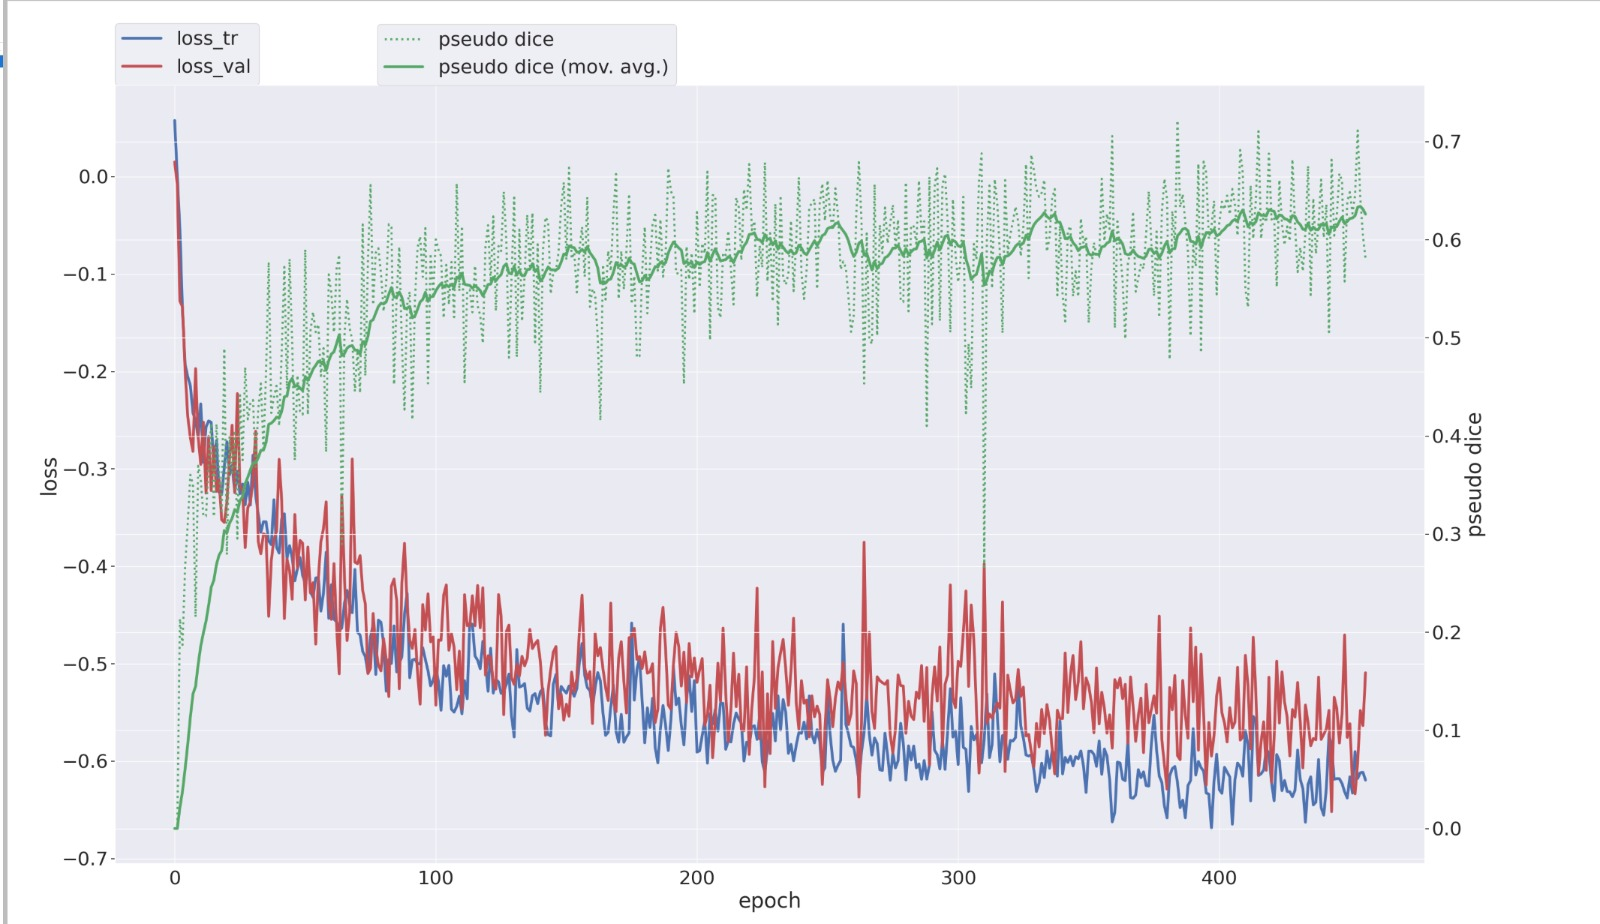
\includegraphics[width=1.0\textwidth]{progress_graph.jpeg}
  \caption{Training progress over 470 epochs. Blue: Training Loss, Red: Validation Loss, Green: Pseudo Dice (validation).}
  \label{fig:progress}
\end{figure}

\begin{table}[h!]
\centering
\caption{Mean results of the model on the validation set (27 cases).}
\label{tab:rezultate}
\begin{tabular}{@{}ll@{}}
\toprule
Metric & Value \\ \midrule
\textbf{Dice (DSC)} & \textbf{0.44616} \\
\textbf{IoU (Jaccard)} & \textbf{0.33019} \\
True Positives (TP) & 6920.56 \\
False Positives (FP) & 6904.81 \\
False Negatives (FN) & 7196.24 \\
True Negatives (TN) & 52,521,137.94 \\
Total Predictions (n\_pred) & 13825.37 \\
Total Reference (n\_ref) & 14116.81 \\ \bottomrule
\end{tabular}
\end{table}

\subsection{Discussion of Results and Examples}

A Dice score of 0.446 is a modest result. It indicates that the model has started to learn the general location and shape of the nodules, but it is far from precise, with less than 50\% overlap with the ground truth.

The high and very similar numbers for False Positives (FP) and False Negatives (FN) show that the model has two main problems:
\begin{enumerate}
    \item It is segmenting regions that are not nodules (FP). % <-- Fixed indentation
    \item It is missing large parts of the actual nodules (FN). % <-- Fixed indentation
\end{enumerate}

This result is expected for two main reasons:
\begin{itemize}
    \item \textbf{The dataset is very small} (108 training images). % <-- Fixed indentation
    \item \textbf{Training was stopped prematurely} at 470 epochs. The default 1000-epoch schedule is designed to let the learning rate decay, which allows the model to refine its predictions. Stopping early means the model is still in a high-learning-rate phase. % <-- Fixed indentation
\end{itemize}

For a qualitative analysis, I used a NIfTI viewer (ITK-SNAP) to overlay the predictions on the CT scans, as shown in Figure~\ref{fig:visualization}. % <-- FIXED: Was \ref{fig:placeholder}

\begin{figure}[htbp]
    \centering
    \begin{subfigure}[b]{0.48\textwidth}
         \centering
         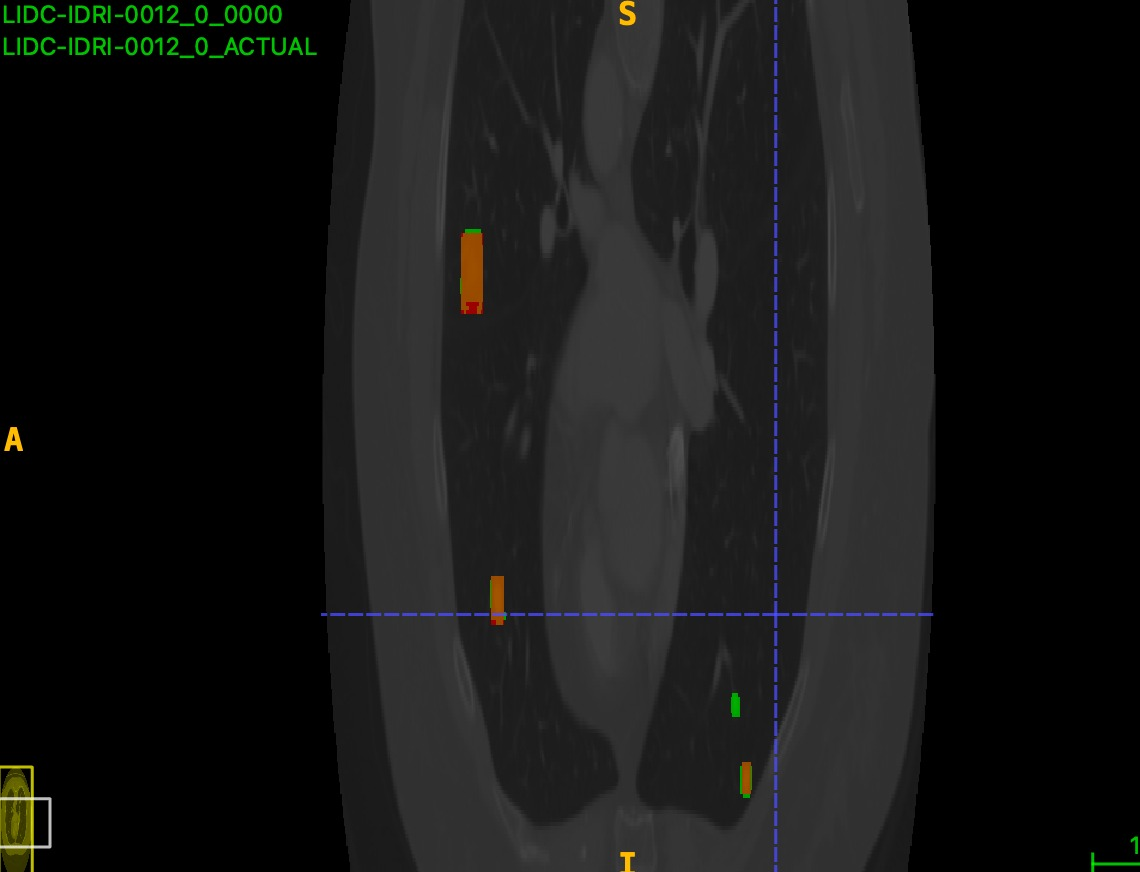
\includegraphics[width=\textwidth]{pred_1.jpeg}
         \caption{View 1}
         \label{fig:view 1}
    \end{subfigure}
    \hfill
    \begin{subfigure}[b]{0.48\textwidth}
         \centering
         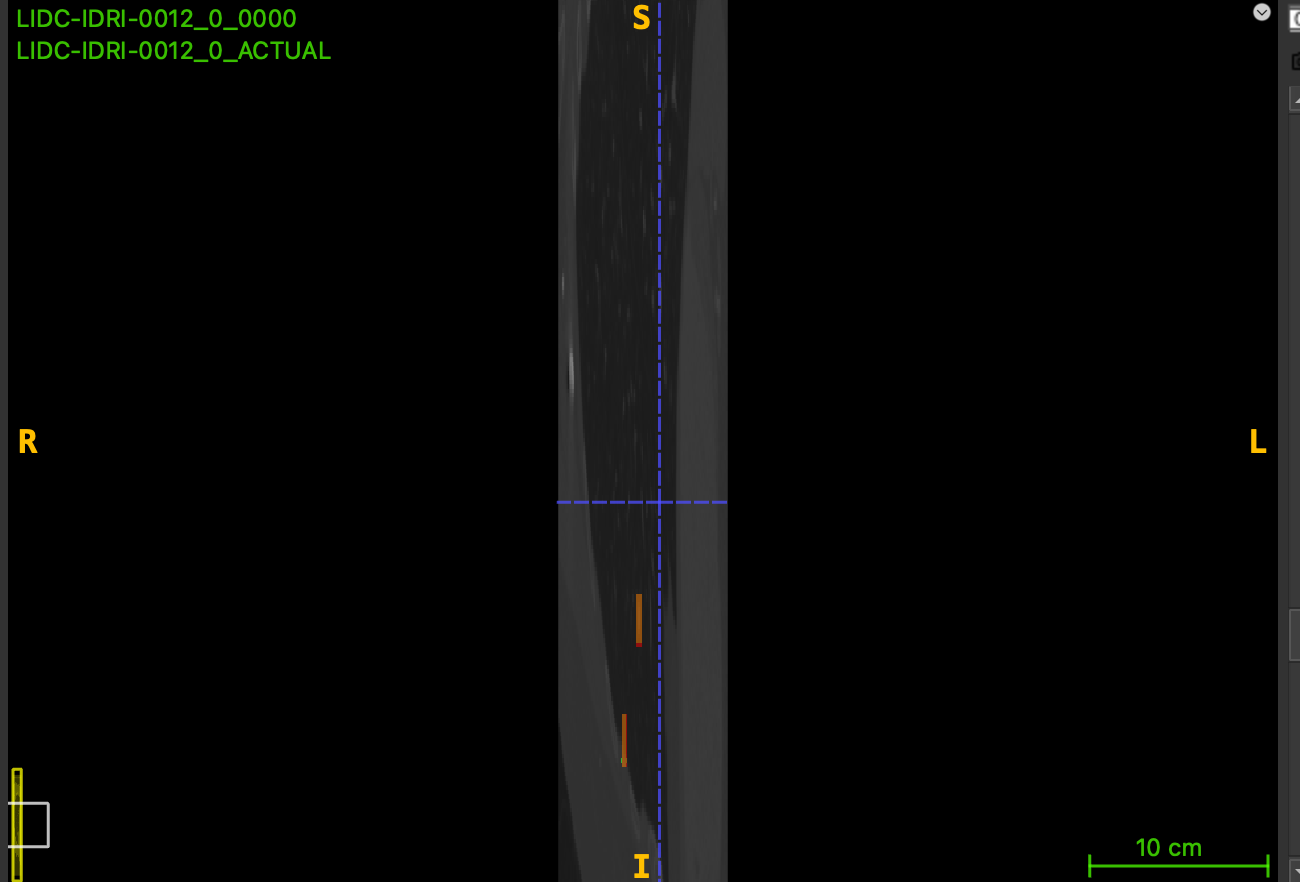
\includegraphics[width=\textwidth]{pred_2.png}
         \caption{View 2}
         \label{fig:view 2}
    \end{subfigure}
    \caption{Qualitative results from the test set (Case LIDC-IDRI-0012). The model's prediction is in green, and the actual ground truth is in red. These images show both hits (good overlap) and misses (green-only or red-only areas).}
    \label{fig:visualization}
\end{figure}

\end{document}